%%%%%%%%% PROJECT DESCRIPTION  -- 15 pages (including Prior NSF Support)

\required{Project Description}
%\begin{center}
%\emph{Maximum of 6 pages}
%\end{center}
%The Project Description (including Results from Prior NSF Support, which is limited to five pages) may not exceed 15 pages. Visual materials, including charts, graphs, maps, photographs and other pictorial presentations are included in the 15-page limitation. PIs be cautioned that the project description must be self-contained and that URLs that provide information related to the proposal should not be used. 

%All proposals to NSF are reviewed utilizing the two merit review criteria, intellectual merit and broader impacts. 

% The Project Description should provide a clear statement of the work to be undertaken and must include: objectives for the period of the proposed  work and expected significance; relation to longer-term goals of the PI's project; and relation to the present state of knowledge in the field, to work in progress by the PI under other support and to work in progress elsewhere.

%%%%%%%%%%%%%%%%%%%%%%%%%%%%%%%%%%%%%%%%%%%%%%%%%%%%%%%%%%%%%%%%%%%%%%
%INTRO
% a brief and informative introduction or background section
%%%%%%%%%%%%%%%%%%%%%%%%%%%%%%%%%%%%%%%%%%%%%%%%%%%%%%%%%%%%%%%%%%%%%

\section*{A. Introduction}	% might be a little long currently, should not repeat the summary page

A critical goal of evolutionary biology today is to understand organisms' abilities to adapt to new or changing conditions. This is especially relevant in the face of global climate change and other increasingly common anthropogenic changes to the environment \citep{Easterling:2000ja}. Many important phenotypic traits are quantitative, and in order to understand the potential for adaptation of these traits and maintenance of variation underlying them, %\jri{not sure the maintenance of variation thing fits well}\kjg{guess I was thinking if fewer loci of larger effect, larger chance of fixing variation?}
we must understand their genetic architecture and how this architecture may be changed as a result of evolutionary processes such as selection and demography. Such knowledge advances our understanding of the process of adaptation and can further benefit crucial goals such as improving crop yields under changing climates. 

Many ecologically or economically important traits have a complex, quantitative genetic basis, and much heterogeneity has been found among these traits in terms of the number of loci contributing to variation, their effect sizes, and their frequencies both within and among species \citep{orr:2001, slate:2005}. Knowledge of this genetic architecture of such traits is important for understanding how easily or quickly local adaptation may occur, or how long and difficult that process may be \citep{Orr:2005dy, Yeaman:2015cc, Yeaman:2011jv}. Such knowledge can therefore greatly contribute to improve breeding and conservation efforts as well as to predicting responses to environmental changes.

%DELETED: considered in the proposed research concern the number of underlying loci and their various effect sizes and dominance relationships. Whether this genetic architecture consists of many loci of small effect or few of large effect can play a role in the impact of demography and selection, as well as mutation, on the genome. How the genome may be restructured as a result of various demographic histories and those effects on selection is not well studied, nor how new genes may evolve to underly traits of importance \citep{Long:2003}. 

The genetic architecture of a trait is determined by a number of factors, including population size, mutation, demographic history, and the history of both purifying and positive selection. Population bottlenecks, for example, can lead to the loss of variation or maintenance of deleterious variation \citep[e.g.][]{Renaut:2015hi, Gunther:2010}. Strong selection, such as that imposed during crop domestication, can fix large-effect loci \citep{Brown:2011}. And recently both theoretical and empirical studies in humans have shown that the types of mutations \citep{Thornton:2013} and the interaction of demographic and selective histories \citep{Fu:2014jt, Gravel:2011iq, Henn:2015dp} have likely changed the genetic architecture of human phenotypes.

%\jri{getting into $N_e$ in the intro is too fast. instead, expand on point from last paragraph here on what we know/don't (see comments in latex)}
Previous studies using genome-wide association (GWAS) and QTL approaches are limited by inability to detect small effect alleles. QTL studies are not able to achieve the resolution necessary for distinguishing the number and effect size of contributing loci, while GWAS studies 
%GWAS and QTL approaches which suffer from limitations due to inability to detect small effect alleles. \jri{i think inclusion of the rockman/mackay studies you mention here would be excellent!!}
% i think many readers will think ``oh another qtl study.''  we should point out the limitations of both qtl and gwas: qtl is too low resolution to identify individual loci, and gwas only tells us what we can find, not what is actually there. so if, for example, lots of causal variants are very rare with large effects, those will be missed by current GWAS (cite Kevin). alternatively, if there are tons of loci each with teeny effects, those may not make genome-wide significance thresholds (cite one of the visscher papers). 

%MOVED: This has implications for studies attempting to identify loci important in adaptation which struggle when each locus out of many may only contribute a small amount to the trait (cite ? Mackay et al Nature Reviews Genetics 10, 565-577 ?, Rockman 2012 Evolution 61:1�17). Thus, studies that aim to identify loci important in adaptation will benefit from knowledge on the range of mutation effect sizes they may expect to see when performing GWAS or genotype-environment associations. 

%DELETED: torsten - rice?). Such bottlenecks greatly decrease the effective population size ($N_e$) which can increase the effect of random genetic drift. The effect size, or strength of selection ($s$), for a given locus, can also impact the efficiency of selection across the genome (selection effective when $N_es>1$). Thus, as demography changes, so does $N_es$ and therefore so does the occurrence of different beneficial, deleterious, or neutral loci across the genome.

My proposed research aims to investigate how these factors shape the architecture of quantitative traits in maize.  Maize and teosinte are extensively studied and serve as ideal models for this research. Maize (\emph{Zea mays}, ssp. \emph{mays}) was domesticated from its wild teosinte ancestor, \emph{Zea mays}, ssp. \emph{parviglumis}, approximately 9,000 years ago in southwestern Mexico \citep{Matsuoka:2002, Piperno:2009}. Thanks to its economic importance and history as a model genetic organism, extensive genomic and phenotypic data exist, making maize an ideal system to in which to study processes affecting genetic architecture.  Previous work, for example, has estimated the demographic impacts \citep{Wright:2005} and identified loci under selection \citep{Hufford:2012dy} during maize domestication. A number of studies have used GWAS to study the architecture of phenotypes of interest in both maize \citep{Wallace:2014} and teosinte \citep{Weber:2009}, allowing us to match simulated and theoretical results with empirical estimates for both taxa.

I propose three objectives which make use of the extensive knowledge and data available in the maize\//teosinte system in order to answer the question of \textbf{how demography and selection change the genetic architecture of quantitative traits}. Objective one builds a simulation model to match the genetic architecture of phenotypically important traits in teosinte. Objective two then simulates the demographic history of teosinte's domestication into modern-day maize and compares the expectations created from simulation to the genetic architecture of modern maize. Objective three further investigates the role of demography and selection on changing genetic architecture by simulating the histories of multiple landraces of maize that spread across the Americas post-domestication. This research will further our understanding of the impact of demography and selection impacts on phenotypic traits, improving our ability to predict the effects of selection and changing environments as well as to exploit genetic diversity in crops for continued breeding.


%%%%%%%%%%%%%%%%%%%%%%%%%%%%%%%%%%%%%%%%%%%%%%%%%%%%%%%%%%%%%%%%%%%%%%
%OBJECTIVES
% a statement of research objectives, methods, and significance
%%%%%%%%%%%%%%%%%%%%%%%%%%%%%%%%%%%%%%%%%%%%%%%%%%%%%%%%%%%%%%%%%%%%%%

\section*{B. Research Objectives, Methods \& Significance}
\subsection*{Objective I: Model the genetic architecture of phenotypes in teosinte}

This first objective aims to build a model to simulate the genetic architecture of phenotypes in teosinte (\emph{Zea mays} ssp. \emph{parviglumis}).  Such a model will then enable us to study how demography and selection during domestication (Objective II) and range expansion (Objective IV) have impacted the genetic basis of phenotypic traits.

In order to model the architecture of quantitative traits, we first need to understand the effects of mutation.  The distribution of fitness effects (DFE) describes the consequences of mutations in terms of their impacts on an organism's fitness. 
%DELETED:Mutations can broadly be classified as beneficial, deleterious, or neutral, but in actuality, mutation effect sizes span a continuum of strongly deleterious to strongly beneficial, with any value in between. %good stuff, but probably not needed

Taking advantage of published \citep{Chia:2012} and new (see Data section below) whole-genome sequencing data in teosinte, we will estimate the DFE in teosinte with the software DoFE \citep{Keightley:2007hq, Stoletzki:2011} using estimates of the number of nonsynonymous and synonymous substitutions in genes.
The resulting estimates of the fitness effects of new mutations can then be parameterized in terms of their effect on a fitness-related quantitative trait  \citep{Keightley:1988, eyre-walker:2010} such as yield, plant height, or flowering time.

%DELETED:Estimate of the DFE and effect size of new mutations will then be used 
%s well as new seqI will apply this method to sequence data from regions of the genome known to underly important phenotypic traits. Some such quantitative phenotypes include yield, plant height, and flowering time, which are of critical importance to agriculture (cite). From this distribution of fitness effects and fitness measures from these traits, we can then translate these values into effect sizes per allele.\kjg{eek, not sure I'm describing this well} I will use genotypic and phenotypic data on teosinte which is available for 5,000 individuals at 16 phenotypic traits (height, kernel traits...\kjg{do you think I should list them all here?}) (cite data source). These individuals are the progeny of 70 teosinte individuals sequenced to 25X coverage, providing an ideal resource for this analysis.

The estimated DFE, combined with prior information on mutation \jri{cite clark 2005 MBE} and recombination rates \jri{cite rodgers-melnick 2015 10.1073/pnas.1413864112}  will then be used as input in simulation models of quantitative trait evolution.  Additional parameters necessary for our model (including dominance and the correlation between a trait and fitness\jri{kevin: other params?}) will be estimated using using an Approximate Bayesian computation approach \jri{cite beaumont 2002}: simulation parameters will be drawn from a prior distribution, and results compared to observed data to estimate the parameters' posterior distributions.  We will take advantage of the library fwdpy (a Python implementation of fwdpp \citealt{Thornton:2014kn} available at \jri{cite github}) to write simulation code that explicitly models a quantitative trait evolving under a model of stabilizing selection. From each simulation, we will then perform genome-wide-association analysis in order to compare with observed data from published (\jri{cite Weber}) and on-going (see Data below) analysis of 16 phenotypic traits in a natural population of teosinte. The ABC approach should allow robust estimation of the necessary parameters from a set of several million such simulations.\jri{do we need more detail on fwdpy? size of region etc? you had this and i commented out.} 

\jri{need final paragraph here, see latex for comments} 
%NEED new paragraph on 1) why having the DFE (which is just distribution of s, not genetic architecture itself) is cool. see eyre-walker NatRevGen 2007. 2) the fact that a model like this currently doesn't exist! no plug-and-play software, very limited theory. so just finishing objective 1 will be awesome!

%DELETED:the genomic architecture desired: distribution of effect sizes across the desired number of loci, including deleterious mutations and their effects on the phenotype. Values of $V_G$, $V_A$, and $V_D$ can be run to equilibrium, and then the populations sampled in order to test for successful replication of a wild teosinte population.

%DELETED:Characterizing the DFE of teosinte and translating this into a distribution of effect sizes uncovers whether the genetic architecture of important quantitative phenotypic traits in teosinte are underlain by many loci of small effect, few loci of large effect, or any combination therein. 
%DELETED:Estimating the DFE in teosinte will further inform a larger body of work aimed at understanding how common different genetic architectures are for traits important in adaptation. The DFE is difficult to estimate and not broadly understood in evolutionary biology for any given organism or in terms of how much it may vary across organisms. This difficulty arises particularly for cases where there are many loci of small effects: such small effect sizes are difficult to detect on an individual basis. 
	
	

%_________________% DATA INFORMATION %_________________%

%%%RARE ALLELES PROJECT (probably the most useful data)
% 1 pop of teo w/ 70 parents (sequenced), 5000 progeny (16 phenotypes, GBS, imputation in progress)
% 1 pop of landrace maize w/ 55 parents (sequencing in progress), 5000 progeny (~25 (?) phenotypes, GBS, imputation in progress)
% 4 additional teo pops,  each with 10 parents (sequencing in progress) and 1200 progeny (GBS done, phenotyping in progress done in Jan 2017)
% 4 additional landrace maize pops,  each with 10 parents (sequencing in progress) and 1200 progeny (GBS done, phenotyping in progress done in Jan 2017)

%%OTHER DATA OF USE
% for teosinte architecture
% Weber 2009 teosinte population (if DNAs still available; may be too small sample size pop) 

%for architecture of traits in maize

% NAM!! 5000 RILs, GBS, 42 phenotypes    26 parents crossed to an additional line, 15 million snps


%(suboptimal) alternative DFE, diversity data
% ~1500 sequnced maize genomes (Hapmap 3 and 4) 

%for comparison of maize and teo architecture
% teosinte synthetic: ~2500 DH lines, ~12% teosinte, 40% B73, 2% of each other 25 NAM parents there is dna and tissue
% Briggs 2007 mapping population (600 BC2S3 to estimate ), maybe genotyped on ~1500 markers
% Sherry parviglumis NILs (~800??) there are seeds

% for looking at other landraces
% ~6 landrace genomes each from highland mexico, lowland mexico, highland S. america, lowland s. america, highland guatemala, US southwest
% SeeDs: 
	% 4,000 landraces each w/ 1M SNPs and several phenos (publicly available)
	% 25,000 landraces, each w/ pooled seq. of ~30 plants. + some phenos (not yet avaible, but we know the woman in charge of the program)
	
% other goodies
% 0.2cM-scale recombination map
% rho-map (starting Feb. 2016)
%___________________________________________________%	
	
\subsection*{Objective II: Model quantitative genetics of maize domestication}

The model developed in Objective I will enable simulation of quantitative traits under stabilizing selection.  Here we will modify this model in to incorporate both demographic change and directional selection, and use it to investigate the impact of domestication on the genetic architecture of phenotypes of interest. Both demographic change associated with a domestication bottleneck and directional selection are expected to change the architecture of quantitative traits, but current theory includes only relatively simple models, and a detailed understanding of how these two forces interact is lacking. 

First, we\jri{i've been writing 'we' but feel free to change to 'i'; shoudl be consistent throughout though} will extend the simulation framework developed in Objective I to include estimates of population size change during the domestication bottleneck and subsequent expansion \jri{cite wright et al. 2005}.\jri{do we need to explain extent of bneck in maize at 5\%??}
Using parameters estimated in Objective I, we will simulate traits in a population undergoing a domestication bottleneck and perform GWAS on the simulated data. This first analysis provides a null expectation of the genetic architecture of traits in the absence of directional selection. We will compare these results to GWAS in both published \jri{cite wallace 2014} and our own on-going analyses of maize data (see Data below). 

Differences between simulations and observed data are informative of the history of selection on phenotypes, and we will again use fwdpy and our ABC approach to estimate the strength of selection on domestication phenotypes. \jri{i don't think this has ever been done except backwards from archaeological data!} I can assess how traits of varying heritabilities have changed over the course of domestication. 
More heritable traits or traits under stronger positive selection may change in different ways than those not under directional selection passing through the bottleneck and I can test if allelic effect sizes have shifted in the distribution's mean or overall shape to more or fewer loci of large effect. \jri{be more specific than 'may change in different ways' if possible. can cite chevin hospital 2008 PMID:18832353 for effect of directional selection on different QTL allele sizes} I will simulate the same quantitative traits used in Objective I.  Traits in maize such as kernel weight and kernel row number are expected to have been selected for improving the species as a crop, while there are no strong reasons to suspect other traits such as total plant height were under selection.  This suite of traits thus provides us with \emph{a priori} predictions on which traits should show differences from our simple demographic simulations.  \jri{maybe add that differences for traits not thought to be under selection might be explained by genetic correlations with other traits? we could test this by estimating G matrix in maize.}

% results may be attributable to parameter values for selection for which we can then reestimate using ABC, and then resimulate the domestication.  Once closely matched, I can make a second comparison of how the genetic architecture changed over time. 
%The distribution of effect sizes established in objective one are used now to simulate the domestication of maize from teosinte. 
%Again using fwdpy, I will simulate the demographic and selective events that occurred during the domestication of maize. A first step to fit the distribution of effect sizes from objective one will use approximate Bayesian computation (ABC) within fwdpy to estimate the most likely distribution of parameters for $V_G$ and $V_A$.\kjg{did I describe this right?} Simulations will follow the genetic architecture of the aforementioned quantitative traits and their accurate genetic architectures through a strong bottleneck of 5\% of its ancestral $N_e$. Regions of the genome in sizes of 100kb can be simulated with assigned fitness values. Population sizes are easily controlled within fwdpy to mirror the ancestral $N_e$ of maize to its estimated size of $\sim$120,000 followed by the domestication bottleneck which was subsequently followed by a large, rapid growth in population size that expanded populations to at least three times as large as the ancestral $N_e$ (cite). 


\begin{SCfigure}
\centering
   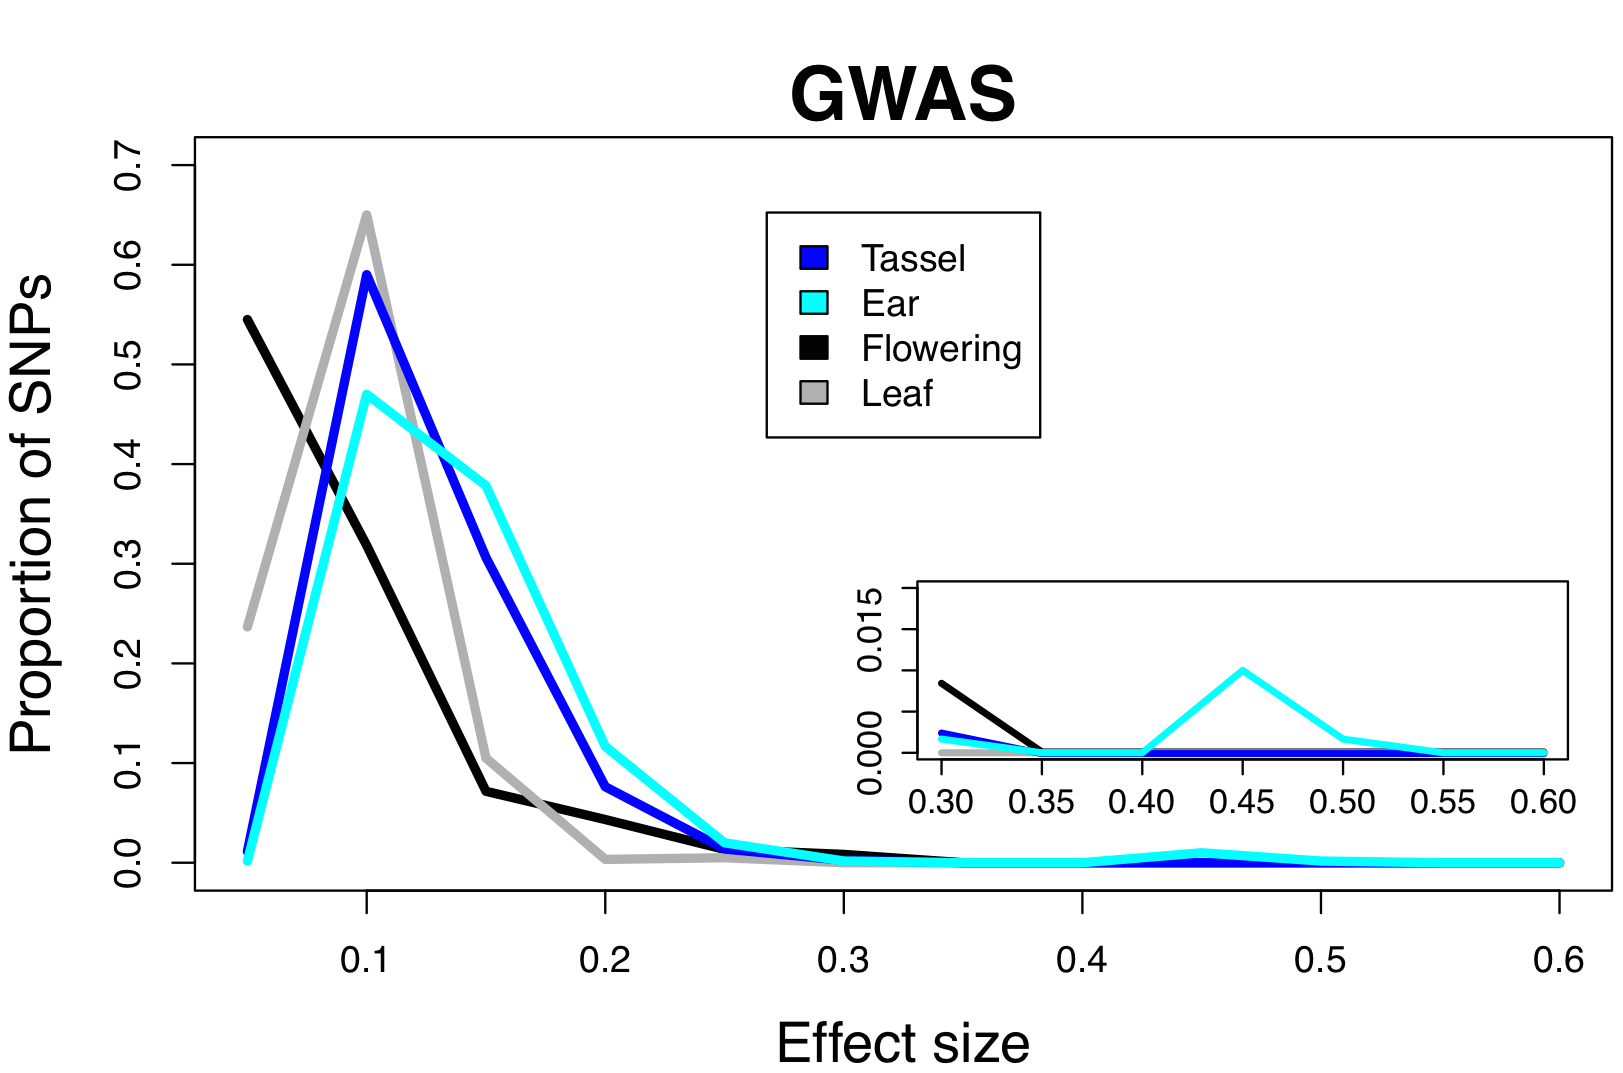
\includegraphics[width=0.7\textwidth]{Figure2_Brownetal2011.png}
  \caption{Effect sizes from GWAS analyses in maize, grouped by trait category. Inset shows the largest effects. Ear traits, showing the largest effect sizes, were likely selected during maize domestication while the others were not. Figure from \citealt{Brown:2011}.}
  \label{fig:model}
\end{SCfigure}

%Having reiterated the origin of modern-day maize in Mexico through simulations, I can now compare the resultant genetic architectures to real genetic architecture in maize data. Genotypic and phenotypic data is currently being generated for another 5,000 progeny individuals of maize, from one landrace of 55 parents (sequenced to 25X) that will be available by the start of this fellowship. Existing data is also available publicly for $\sim$1500 maize genomes through the HapMap 3 and 4 projects (cite) if any unforeseen causes slow the availability of this dataset. 


The results of this objective will show the relative importance of demography and selection in determining maize's genetic architecture. Demographic bottlenecks are common during the geographic spread of populations (cite) and can have several effects on the genome including purging of deleterious alleles (recessive alleles become homozygous and are more efficiently removed), or alternatively may lead to an increase of some deleterious alleles through increased random genetic drift (allele surfing, \citealt{Klopfstein:2005bl}). The effects of these processes varies depending on the degree of population size reduction and the length of time over which populations are bottlenecked (cite bottleneck lit), but also have the potential to interact with the strength of selection during this demographic process. Changes in the distribution of allele effect sizes are not well understood in any system and are controversial in humans \citep{Lohmueller:2014dn, Simons:2014fj, Hancock:2011jb}. Deleterious alleles likely play a large role in many adaptive phenotypes: crop plants have undergone dramatic demographic shifts, usually involving a domestication bottleneck followed by expansion as cultivation spread, and some authors even argue that selection on domestication traits has inadvertently increased the frequency of alleles deleterious for other phenotypes \citep{Gunther:2010}. Consistent with this, it has recently been shown that genes associated with a number of quantitative traits in maize are enriched for deleterious alleles compared to randomly chosen genes \citep{Mezmouk:2014jd}. Such information is crucial for understanding variation in phenotype, designing breeding strategies, utilizing diversity from wild relatives, or even engineering new traits using biotechnology. \jri{this paragraph is great. not sure if it goes here or in project significance?}

\subsection*{Objective III: Validate model predictions in synthetic mapping populations}

Furthermore, a validation of the distributions of fitness effects in maize and teosinte can be performed using data from a synthetic cross of maize and teosinte. This \emph{Zea} synthetic results from a mix of 26 maize lines with 12\% teosinte genes (from 11 different founders, fully sequenced), 40\% B73 (the reference genome line), and 2\% from 25 other inbred maize lines. Using this genomic data to again estimate a distribution of effect sizes for the same traits, but now across regions of the genome known to originate from either maize or teosinte, I can test if the respective distributions for maize and teosinte are recovered in the same genetic background. This will identify if our simulations were truly valid. \jri{expand this a bit, cite Sherry's NIL population too}

\subsection*{Objective IV: Investigate the impact of various demographic and local adaptation of maize landraces maize across the Americas} 

%Maize originated approximately 9,000 years ago in southern Mexico (cite Matsuoka et al 2002, others?) during a single domestication event of \emph{ssp. parviglumis}. Archaeological records also confirm this dating and single location (cite) as well as the subsequent spread and growth in population size of domestic landraces across the Americas into both lowland and highland environments [cite Wilkes, H. G. (1967) Teosinte: The Closest Relative of Maize (Harvard Univ., Cambridge, MA)]. South American landraces of maize also underwent a second bottleneck event during their expansion (cite). Using genetic data, the precise demographic parameters of this history have been estimated (cite Beissinger et al in prep). This provides information on the ancestral effective population size of maize ($N_a \approx$ 120,000), the size to which the population was bottlenecked during domestication (5\% of this $N_a$), the subsequent size to which populations rapidly expanded (3 times as large as $N_a$\kjg{but maybe as much as 1E9, citation}), and lastly on the genome-wide mutation rate ($3.8\times10^-8$ cite Clark et al 2005 MBE 22, 2304 -- 2312.)


Since domestication, various landraces of maize have spread across Central and South America and adapted into different lowland and highland habitats.\kjg{worth a figure? am short on space already} These populations have experienced further demographic and selective pressures in addition to the initial domestication bottleneck. South American populations are inferred to have experienced a second severe bottleneck (cite), populations expanding geographically are likely to have experienced serial founder effects that can change allele frequencies in unexpected ways due to allele surfing \citep{Klopfstein:2005bl}, and gene flow between teosinte and maize populations may have continued in some cases. Selection pressures in different lowland and highland habitats may also interact with these demographic events.

The objective of this project is to simulate the impact of multiple demographic events and selective pressures either individually or in combination. This will show how much variation is possible in terms of the effects on genetic architecture underlying traits for adaptation. The core set of simulations in this project will be designed to match the known landraces in maize, but will include more broadly a designed experiment to compare the presence or absence of particular evolutionary forces. Though there is currently not sufficient genomic and phenotypic data for all landrace populations of maize, it is likely that this will exist in the future, leaving an excellent future comparison to be made in terms of how well these simulation results match real populations across the species range. The goal of this project is to inform our understanding of the relative importance or insignificance of the tested demographic cases and how sensitive genetic architecture is to these. There is a debate currently in the field of evolutionary biology and human demographic history about the impact of events such as range expansions on the genome and the frequency of deleterious alleles \citep{Henn:2015ce, Sudmant:2015}, necessitating further understanding of how such factors might interact under various selective environments. Furthermore, deleterious alleles likely play a large role in many adaptive phenotypes: crop plants have undergone dramatic demographic shifts, usually involving a domestication bottleneck followed by expansion as cultivation spread, and some authors even argue that selection on domestication traits has inadvertently increased the frequency of alleles deleterious for other phenotypes \citep{Gunther:2010}. Consistent with this, it has recently been shown that genes associated with a number of quantitative traits in maize are enriched for deleterious alleles compared to randomly chosen genes \citep{Mezmouk:2014jd}. Such information is crucial for understanding variation in phenotype, designing breeding strategies, utilizing diversity from wild relatives, or even engineering new traits using biotechnology. 

Similar to objective two, I will simulate regions of the genome within individuals known to underly important phenotypic traits. These individuals will occupy populations that will be subjected to combinations of demographic and selective pressures including some of the following. To recapitulate the various landraces of maize, I will include cases of a second bottleneck after the domestication bottleneck, populations undergoing little or significant additional range expansion (Central American versus South American), stronger or weaker selection on flowering time and phenological traits (warmer lowland versus colder highland adapted populations), and cases with or without gene flow from sympatric\kjg{is that accurate, there is teosinte around them at least?} populations of teosinte. I will do additional simulations to cover a wider range of parameters covering these cases, i.e. more extremes of a longer or larger range expansion, stronger and weaker bottlenecks, and higher or lower levels of gene flow among populations. This will allow assessment of how important the details of demography are in determining the genetic architecture of local adaptation to different conditions.\kjg{feel like I kind of repeated myself at the end here, maybe move the methods in earlier?}

\subsection*{Data}
This project will make use of both published data as well as data generated or currently being generated as part of a related Plant Genome project (Biology of Rare Alleles IOS-1238014) of which sponsoring scientist Dr. Ross-Ibarra is a Co-PI. As part of this project, Dr. Ross-Ibarra's group is currently in the process of sequencing 70 teosinte and 55 maize genomes to high depth. These genome sequences should be finished by the end of 2015 and will be made publicly available early 2016 via the group website (\url{www.panzea.org}). The individuals used for genome sequencing are also the parents of two large mapping populations of $\approx 5000$ progeny. Both populations have been genotyped and phenotyped for a number of traits including seed yield, flowering times, and plant height.  These data are currently available via collaborators.  Publication of results from analyses of these data must await publication of collaborators' GWAS analyses, but but as these currently underway and comparisons of simulations in Objectives I and II would not begin until early 2017 at the soonest we do not foresee this being an issue. \jri{jri todo: add mention of zea synthetic}

Objective IV of this project... \jri{do we want to include the SeeDs phenotype/genotype data?}
	
%%%%%%%%%%%%%%%%%%%%%%%%%%%%%%%%%%%%%%%%%%%%%%%%%%%%%%%%%%%%%%%%%%%%%%
%TRAINING OBJECTIVES
% training objectives and plan for achieving them (these may include scientific as well as other career preparation activities)
%%%%%%%%%%%%%%%%%%%%%%%%%%%%%%%%%%%%%%%%%%%%%%%%%%%%%%%%%%%%%%%%%%%%%%
\section*{C. Training Objectives}

This fellowship will provide me with an ideal opportunity to learn the skills needed to enhance my ability to conduct cutting edge research in the fields of genomics and computational biology, both areas in which I expect to continue my future research and which are greatly expanding in evolutionary biology. I will gain many skills related to genomic data analysis through these projects, learning bioinformatics and analysis skills for large datasets. I have limited experience working with genomic data from my dissertation, thus making this a vital step in my career. Genomic technology and data are growing at an incredibly fast pace, and working directly with such data will teach me the most up to date, accurate, and efficient approaches. I will also improve my computational biology skills through the proposed simulations, learning a new and useful programming language, Python, that I can apply throughout this research and my future research in evolutionary biology. 


%%%%%%%%%%%%%%%%%%%%%%%%%%%%%%%%%%%%%%%%%%%%%%%%%%%%%%%%%%%%%%%%%%%%%%
%CAREER DEVELOPMENT
% an explanation of how the fellowship activities will enhance your career development and future research directions as well as describing how this research differs from your dissertation research, thus providing you an opportunity to broaden your scientific horizon
%%%%%%%%%%%%%%%%%%%%%%%%%%%%%%%%%%%%%%%%%%%%%%%%%%%%%%%%%%%%%%%%%%%%%%
\section*{D. Career Development \& Future Research}

My career goal is to develop an innovative research program in evolutionary biology, studying population genetics and the processes that impact genetic diversity. I believe such research is key for the future, not only for the field of evolutionary biology, but also in applied scenarios such as understanding prevalence of genetic diseases in humans, adaptation of species to climate change, or strategies for improving agricultural products for a growing world population. My dissertation research has approached some of these questions in a more theoretical and less applied mindset. The work I will conduct during this fellowship would have more direct potential for application in the field of maize agriculture. For me, this is necessary and vital experience for my career development as I decide between pursuing a more applied research program, potentially in industry or government research scientist positions, or in pursing a career as an academic researcher at a university.

The skills I will develop during this fellowship, as described in section C, will benefit my career and put me on the cutting edge for analyses of the newest genomic data and the most recent computational approaches for biological simulations. Interacting with Dr. Ross\--Ibarra, as well as other researchers at UC Davis, and with Dr. Kevin Thornton at UC Irvine, will be both intellectually stimulating and rewarding experiences that will help me accomplish my career goals. Drs. Ross\--Ibarra and Thornton are both at the forefront of a popular movement for open science, making all stages of the research process transparent to any interested parties, and providing products such as data and code immediately and publicly. This is a work ethic I strongly agree with and hope to contribute to as an independent researcher. Our work together will better equip me with the tools and experience that make open science easy, efficient, and profitable\jri{unfortunate word choice. rewarding?} for all. I believe that this will equip me as a competitive, knowledgeable, and independent researcher able to conduct interesting and useful research throughout my future research program on topics of local adaptation, demographic history, population structure and genetic architecture of important traits. Furthermore, Dr. Ross-Ibarra has an excellent track record of helping his post-doctoral fellows secure promising positions for their future careers, including 3 assistant professorships at universities, 2 research scientist positions in the seed industry, one at an NGO, and one in the USDA. 

%%%%%%%%%%%%%%%%%%%%%%%%%%%%%%%%%%%%%%%%%%%%%%%%%%%%%%%%%%%%%%%%%%%%%%
% HOST INSTITUTION
% a justification of the choice of sponsoring scientist(s) and host institution(s)
%%%%%%%%%%%%%%%%%%%%%%%%%%%%%%%%%%%%%%%%%%%%%%%%%%%%%%%%%%%%%%%%%%%%%%
\section*{E. Sponsoring Scientists and Host Institution}

The University of California Davis (UCD) is the ideal place to conduct the proposed research. UCD has a world-renowned program in evolutionary biology and faculty in population genetics who are at the top of the field. Jeff Ross\--Ibarra is an expert on teosinte, maize, its domestication, and the associated population genetics and genomics of the system. \kjg{Jeff, feel free to make that sound better} 
Kevin Thornton is an accomplished quantitative geneticist and computational biologist at UC Irvine, who will also contribute greatly to this research. \kjg{Likewise Kevin, feel free to modify}
They will both serve as effective and capable mentors for my post-doctoral research. In particular, Jeff has been studying the maize\//teosinte system for many % maybe being vague is okay, or you want to remove entirely? \emph{XX}\kjg{don't forget to fill in}\jri{only 6! i think we sholdn't cite since that doesn't sound like a lot} 
years with a great network of collaborators providing vast resources of data. His work has contributed largely to our knowledge of this system, and more generally on domestication and adaptation as evolutionary processes. Kevin is also the developer and maintainer of fwdpy, the python package proposed for completing the simulations. He will thus serve as a great resource in terms of knowing the exact capabilities of the simulation method and any assumptions of its model that must be taken into account.
Furthermore, the Department of Ecology and Evolution, the Department of Plant Biology, and the Department of Plant Sciences at UCD have many exceptional faculty doing research relevant to my interests, providing many research groups to interact with on a daily basis for potential collaborations or feedback on this research. For example, I look forward to interacting with scientists interested in population genetics, such as Graham Coop, and in adaptation, such as Johanna Schmitt. %Additionally, experts in plant regulatory evolution, such as Neelima Sinha, Siobhan Brady, and Daniel Runcie will serve as great people to interact with. % need to look up people in the dept, these names were just taken from Emily J's application
UCD has the necessary computing resources for our proposed work, and as described, vast sources of knowledge and experience on the topics I plan to investigate, ensuring the success of this work. I am excited to join and contribute to UCD's active and vibrant scientific community. \jri{should probably add something about Farm and Kevin's cluster}


%%%%%%%%%%%%%%%%%%%%%%%%%%%%%%%%%%%%%%%%%%%%%%%%%%%%%%%%%%%%%%%%%%%%%%
%Milestones
% a timetable with yearly goals with benchmarks for major anticipated outcomes
%%%%%%%%%%%%%%%%%%%%%%%%%%%%%%%%%%%%%%%%%%%%%%%%%%%%%%%%%%%%%%%%%%%%%%
\section*{F. Milestones \& Timeline}
\begin{tabular}{ll}
Year 1: & Estimate DFE in teosinte; design model \& perform ABC (Obj. I) \\
Year 2: & Model domestication \& selection, validate with empirical data (Obj. II, III)\\
Year 3: & Model local adaptation, population expansion (Objective IV).  \\
\end{tabular}

%%%%%%%%%%%%%%%%%%%%%%%%%%%%%%%%%%%%%%%%%%%%%%%%%%%%%%%%%%%%%%%%%%%%%%
%BROADER IMPACTS
% a separate section within the narrative that describes in detail the broader impacts of the proposed activities.
%%%%%%%%%%%%%%%%%%%%%%%%%%%%%%%%%%%%%%%%%%%%%%%%%%%%%%%%%%%%%%%%%%%%%%
\section*{G. Broader Impacts}

The proposed research will have wide-ranging impacts for both the public and the scientific community. I will ensure that my results are available to the public at all stages of these projects by maintaining code and scripts online at my GitHub account, which will allow other researchers to access analysis methods or data cleaning tools as well as simulation details and parameters which can provide a building block from which further research can be conducted. I will present new findings at international conferences and submit publications to open-access pre-print servers. I will also be able to broadcast my work more widely to the public through a strong online presence I maintain on Twitter and \href{http://www.molecularecologist.com/}{The Molecular Ecologist}, a blog I have contributed to in the past. The impacts of this research on corn as a crop species useful for both food and fuel resources is also of an innate broad impact, as understanding the genetics underlying adaptation will ensure a viable future for such crop species in the future. Lastly, this research will contribute greatly to my own career development, improving my knowledge on genomics and working in an economically important crop species. I will be able to learn these vital tools as well as to teach them to undergraduate students in the lab and into the future as the field of genomics continues to grow.\jri{big thing missing here is outreach etc. blogs/twitter a good start, but perhaps offer a workshop, produce other online content? here they are looking for how your work will impact others. examples in the summary doc are a good start too!}


genetic architecture underlying traits affects how easy/hard and quick/slow local adaptation can occur. important for breeding, conservation, predicting response to climate change, etc.
useful info for crops/domesticated species (and also things like disease in humans?) \jri{i think pointing out this is important for humans too is useful in the proj. significance section }


\begin{comment}
Quantitative phenotypes such as yield, plant height, and flowering time are of critical importance to agriculture.  
Deleterious alleles likely play a large role in many of these phenotypes: crop plants have undergone dramatic demographic shifts, usually involving a domestication bottleneck followed by expansion as cultivation spread, and some authors even argue that selection on domestication traits has inadvertently increased the frequency of alleles deleterious for other phenotypes (cite gunther2010). 
Consistent with this hypothesis, my lab has recently shown that genes associated with a number of quantitative traits in maize are enriched for deleterious alleles  compared to randomly chosen genes (cite mezmouk2014).
However, while we know that demography impacts the frequency of individual deleterious variants, we have a poor understanding of the interaction of demography and selection on phenotypic variation. 
In particular, we know little about how these two forces interact to determine the genetic architecture -- the number of genes and their effect -- of a trait. 
Such information is crucial for understanding variation in phenotype, designing breeding strategies, utilizing diversity from wild relatives, or even engineering new traits using biotechnology. 
\end{comment}




